Die API basiert hauptsächlich auf dem Framework \texttt{Microsoft.Entity\-Framework\-Core}.
Ein Objekt vom Typ \texttt{IHost} (Host) mit einer \texttt{IConfiguration} (Konfiguration) schafft die Grundlage der API.
Welche API-Controller eingebunden sind, die Anbindung der Datenbank sowie die Definition der Zugriffsrechte sind Informationen, die in der Konfiguration enthalten sind.

Das bereits im Framework eingebaute Werkzeug \emph{SwaggerUI} kann verwendet werden, um den Aufbau der API grafisch darzustellen und Anfragen direkt über den Browser stellen zu können.
Hier werden auch Definitionen, Kommentare und Datentypen beschrieben und wie sie in der API verwendet werden können.

Das verwendete Datenbanksystem ist SQLite.
Benutzer und Anwendungsdaten werden in zwei getrennten .db-Dateien gespeichert.
Der Grund für diese Trennung liegt in der Funktionsweise der Anbindung.
Während für die Datenbank mit den Anwendungsdaten ein Klasse vom Typ \texttt{DbContext} verwendet wird, benötigt die Verarbeitung der Benutzer und Rollen einen \texttt{IdentityDbContext}.

Damit es hier nicht zu Migrationsproblemen kommt und die Benutzerdaten bei einer Änderung der Datenstruktur  nicht erneut generiert werden müssen, wurden die beiden Kontext-Klassen nicht zusammengelegt.
Außerdem macht diese Methode es möglich, Anwendungsdaten und Benutzerdaten an getrennten Orten aufzubewahren, was im Sinne der Datensicherheit und des Datenschutzes ist.

Die Klassen für Benutzer- und Rollendaten werden von den beiden Frameworks \texttt{Microsoft.\-AspNetCore\-.Identity} und \texttt{Microsoft.\-AspNetCore.\-Identity.\-Entity\-Framework\-Core} bereitgestellt. 
Die Eigenschaften und Beziehungen der Anwendungsdaten können Abbildung \vref{data-erm} entnommen werden.

\begin{figure}[ht]
	\centering
	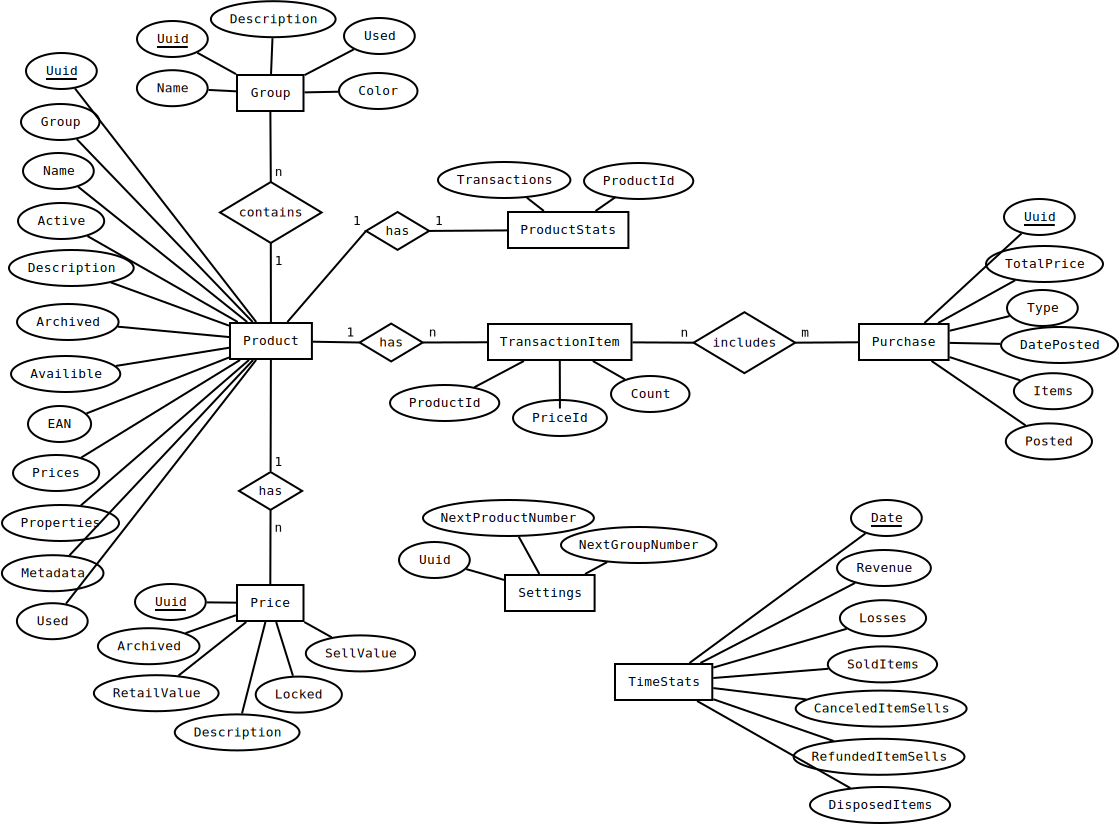
\includegraphics[width=1\linewidth]{ERM.png}
	\caption{ERM der Anwendungsdaten}
	\label{data-erm}
\end{figure}

Damit Endpunkte verwendet werden können, muss sich der Benutzer dafür authentifizieren. 
Dieser Vorgang wird in Abbildung \vref{login-struct} beschrieben.

\begin{figure}[ht]
	\centering
	\includegraphics[width=0.7\linewidth]{Anmeldevorgang.png}
	\caption{Ablauf der Anmeldung}
	\label{login-struct}
\end{figure}